\documentclass[crop,tikz,pgf]{standalone}

\usetikzlibrary{arrows,automata,positioning}

\begin{document}
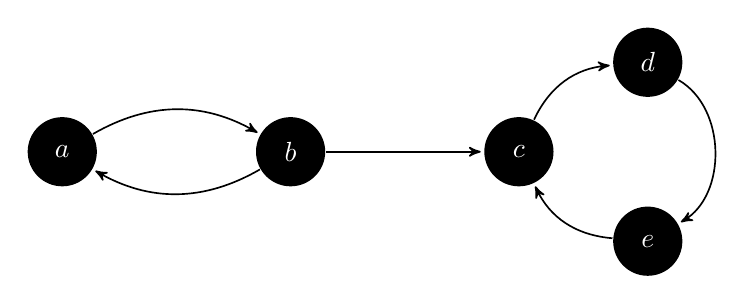
\begin{tikzpicture}[->,>=stealth',shorten >=1pt,auto,node distance=2cm,semithick]
	\tikzstyle{every state}=[fill=black,draw=none,text=white]

	\node[state] (A) {$a$};
	\node[state] (B) [right = of A] {$b$};
	\node[state] (C) [right = of B] {$c$};
	\node[state] (D) [above right = 0.5 and 1 of C] {$d$};
	\node[state] (E) [below right = 0.5 and 1 of C] {$e$};

	\path (A) [bend left] edge (B);
        \path (B) [bend left] edge (A);
        \path (B) edge (C);
        \path (C) [bend left] edge (D);
        \path (E) [bend left] edge (C);
        \draw (D) to [out=330,in=30,looseness=1] (E);
\end{tikzpicture}
\end{document}